\chapter{Modeling stability \& change}\label{ch:Models-of-Change}

In many implemented exemplar models that include production, unbounded
iterative biasing is prevented via the elimination of tokens that
fall in the ambiguous region between two existing categories (\citealt{Wedel2004,Wedel2006,Wedel2008,Blevins2009,DBLP:journals/corr/Tupper14a}).
If the categories are taken to be words, then discarding ambiguous
tokens acts to maintain a meaning distinction that relies on a minimal
sound distinction along the given phonetic dimension. The idea that
sound changes which result in homophony are dispreferred in some way, 
has existed within historical linguistics for a long time (e.g. \citealt{Martinet1955}).
In recent years this notion has been revived and quantified as an
inverse correlation between the probability of a sound change that
neutralizes contrast \emph{x}, and the number of words that are differentiated
only by contrast \emph{x}. This is known as the \emph{functional load}
of the contrast\footnote{There are many other ways one might define functional load. However,
it turns out that a simple minimal pair count seems to be the most
useful of these.} (\citealp{Surendran2006,wedel2013high}). In \citet{Wedel2008},
contrast maintenance (homophone avoidance) is implemented as a storage
probability that is proportional to goodness of fit. Tokens that are
less prototypical members of both categories have a lower probability
of being retained in either category. Thus, as ambiguous tokens are
lost, the two categories are effectively pushed apart. Functional
load can be modeled as a weighting factor in this type of model, increasing
the probability that ambiguous forms will be discarded, and effectively
strengthening the contrast maintenance effect for certain words (\citealt{Soskuthy2015}).

The existence of a second contrasting category along the biasing dimension
will prevent the biased category from moving past a certain point,
allowing the basic exemplar models of the previous chapter to converge.
The assumption of such a category, however, limits the types of sound
changes that can be modeled; in particular, a sound change in which
a new category is formed, presumably from the biased variants of an
existing category. It is exactly this change that is adopted as the
modeling gold standard in this book. Therefore, we will have to consider
what other forces can achieve stability, forces that, if general,
must be included in all models, whether they are implementationally
necessary or not\footnote{A goodness-of-fit function that doesn't directly reference contrast
is possible in this scenario. However, it will not produce the desired
effect for a single category. If prototypicality is determined by
distance from the category mean, then what is acceptable will change
as the mean of the category changes, which will occur because of the
constant phonetic bias. Therefore, the category will move unboundedly.
On the other hand, if prototypicality depends on some fixed value,
then the category will not be able to shift beyond the specified limit
of ``goodness''. }. In this chapter we will analyze, in detail, the consequences of
adding production targets to the basic exemplar models of Chapter
\ref{ch:The-Exemplar-Model}. In doing so we will arrive at a subset
of models that meet the two criteria of boundedness and theoretical
coherence. The full range of possible outcomes for this set of models
will then be derived, setting the stage for an investigation of what
type of architecture would be sufficient (and possibly necessary)
to produce (under the appropriate conditions) the genesis of a new
phoneme category.

It should be noted at this point that it is widely acknowledged that
sociolinguistic factors play a central role in language change. A
class of ``innovators'' may be required, aided by a class of ``early
adopters'' in the actuation and spread of a change (\citealt{milroy1985linguistic}).
Change may require those with less social power to pay more attention
to the speech of those with more power, leading to incorrect inferences
about the source of phonetic variation (e.g. \citealt{Garrett2013}).
Change may require systematic differences between individual speakers
in their analysis of ambiguous data, the degree to which they compensate
for phonetic biases, or some other facet of speech processing (e.g.
\citealp{Beddor2009,yu2013socio}). This paper does not explicitly
address these aspects of sound change in that it focuses on the mental
grammar of a single individual. The approach taken here, however,
is not incompatible, nor inconsistent, with a theory of sound change
that includes socio-indexical variables.

\section{Articulatory targets}

Many of the set of proposed universal phonological features specify
articulatory parameters, such as where in the mouth the tongue tip
makes contact during the production of the sound. Explicit targets
of this kind are often assumed to be unnecessary in exemplar modeling,
where categories are taken to be emergent – dependent only the interaction
of competing forces. This assumption is aided by the practice of treating
the initial distribution of tokens as arbitrary and independent of
the model. A number of works have demonstrated that from a single
global pressure, such as avoidance of homophony, structured categories
can evolve (\citealt{Boer2000,Wedel2006,soskuthy2013phonetic}). However,
sound categories, once established, are unlikely to be determined
solely by the number of contrasts in a given language. If this were
the case, then a category would be defined only by its individual
members (the label {/p/}, for example, would be completely
arbitrary, and contain no information about the use of the lips in
the production of the sound). Furthermore, we would not expect the
consistent phonetic differences that are found in the production of
phonologically identical sounds across different languages (\citealt{Keating1985}).
Distributions would also be predicted to spread out on dimensions
lacking a contrastive segment distinction. Although there is evidence
that the absence of contrast leads to greater variation in pronunciation
along that dimension (e.g. \citealt{choi1995acoustic}), this variation
is not unlimited. \citet{Baker2011}, for example, found a number
of differences in how speakers produced American English “r”
sounds. However, those differences resulted in little to no acoustic
difference between productions. Despite the fact that English does
not contrast different types of rhotic segments, productions do not
expand to fill that large phonetic space. 

\section{\label{subsec:Soft-Targets}Soft targets}

From a purely implementational perspective, production targets offer
a mechanism for avoiding unbounded shift and neutralization. Fixed
targets, however, will prevent any kind of change, and render the
exemplar architecture superfluous. In this section, what amounts to
a semi-fixed target is adopted: a force that acts to keep tokens at
a fixed location, but from which they can be perturbed to some degree
by the usual biasing forces. 

The semi-fixed, or “soft”, duration target is expressed in (\ref{eq:Inertia Force}),
where $\beta$ is a constant between 0 and 1 that determines the strength
of the target, and \emph{N} is the location of the target along the
biasing dimension \emph{x}.
\begin{equation}
I(x_{i})=\beta(N-x_{i})\label{eq:Inertia Force}
\end{equation}
When the category is instantiated with a mean at \emph{N} ($z=0$),
$I(x_{i})$ can be conceptualized as a type of inertia, acting to keep
tokens in place. The further a token moves from the target, the stronger
the force pulling it back. This has the desired effect of bounding
movement in either direction, while still allowing the category to
shift as a whole. If \emph{I} is the only force acting, then the tokens
will eventually settle at the equilibrium point \emph{N}, where the
change in \emph{$\overline{x}$} is 0. \emph{N} can also be characterized
as the optimum of a function with a positive derivative when \emph{x}
is less than \emph{N}, and a negative derivative, when \emph{x} is
greater than \emph{N}. Regardless of the location of \emph{x}, it
is always being pushed in the direction of \emph{N}. 

The Soft Target model is built directly from the gradient context-dependent
model of \sectref{subsec:Model-2:-Lengthening}. Tokens selected
randomly to occur in a biasing context are subjected to a bias that
increases their value along dimension \emph{x} by a small percentage
($\alpha$) of their current value: 
\begin{equation}
L(x_{i})=\alpha x_{i}\label{eq:Lengthening Force}
\end{equation}

Figure \ref{fig:Model2:LengtheningProcess} shows the effect of adding
a soft target to Model 2. Change is constrained relative to the basic
model. This model is also theoretically interpretable; there is a
single category, with a single production target corresponding to
the non-biased segment, and the biasing process applies to all tokens
of this category with equal probability. These properties will become
important as we continue to explore the modeling space in the following
sections. 

\begin{figure}[H]
\centering{}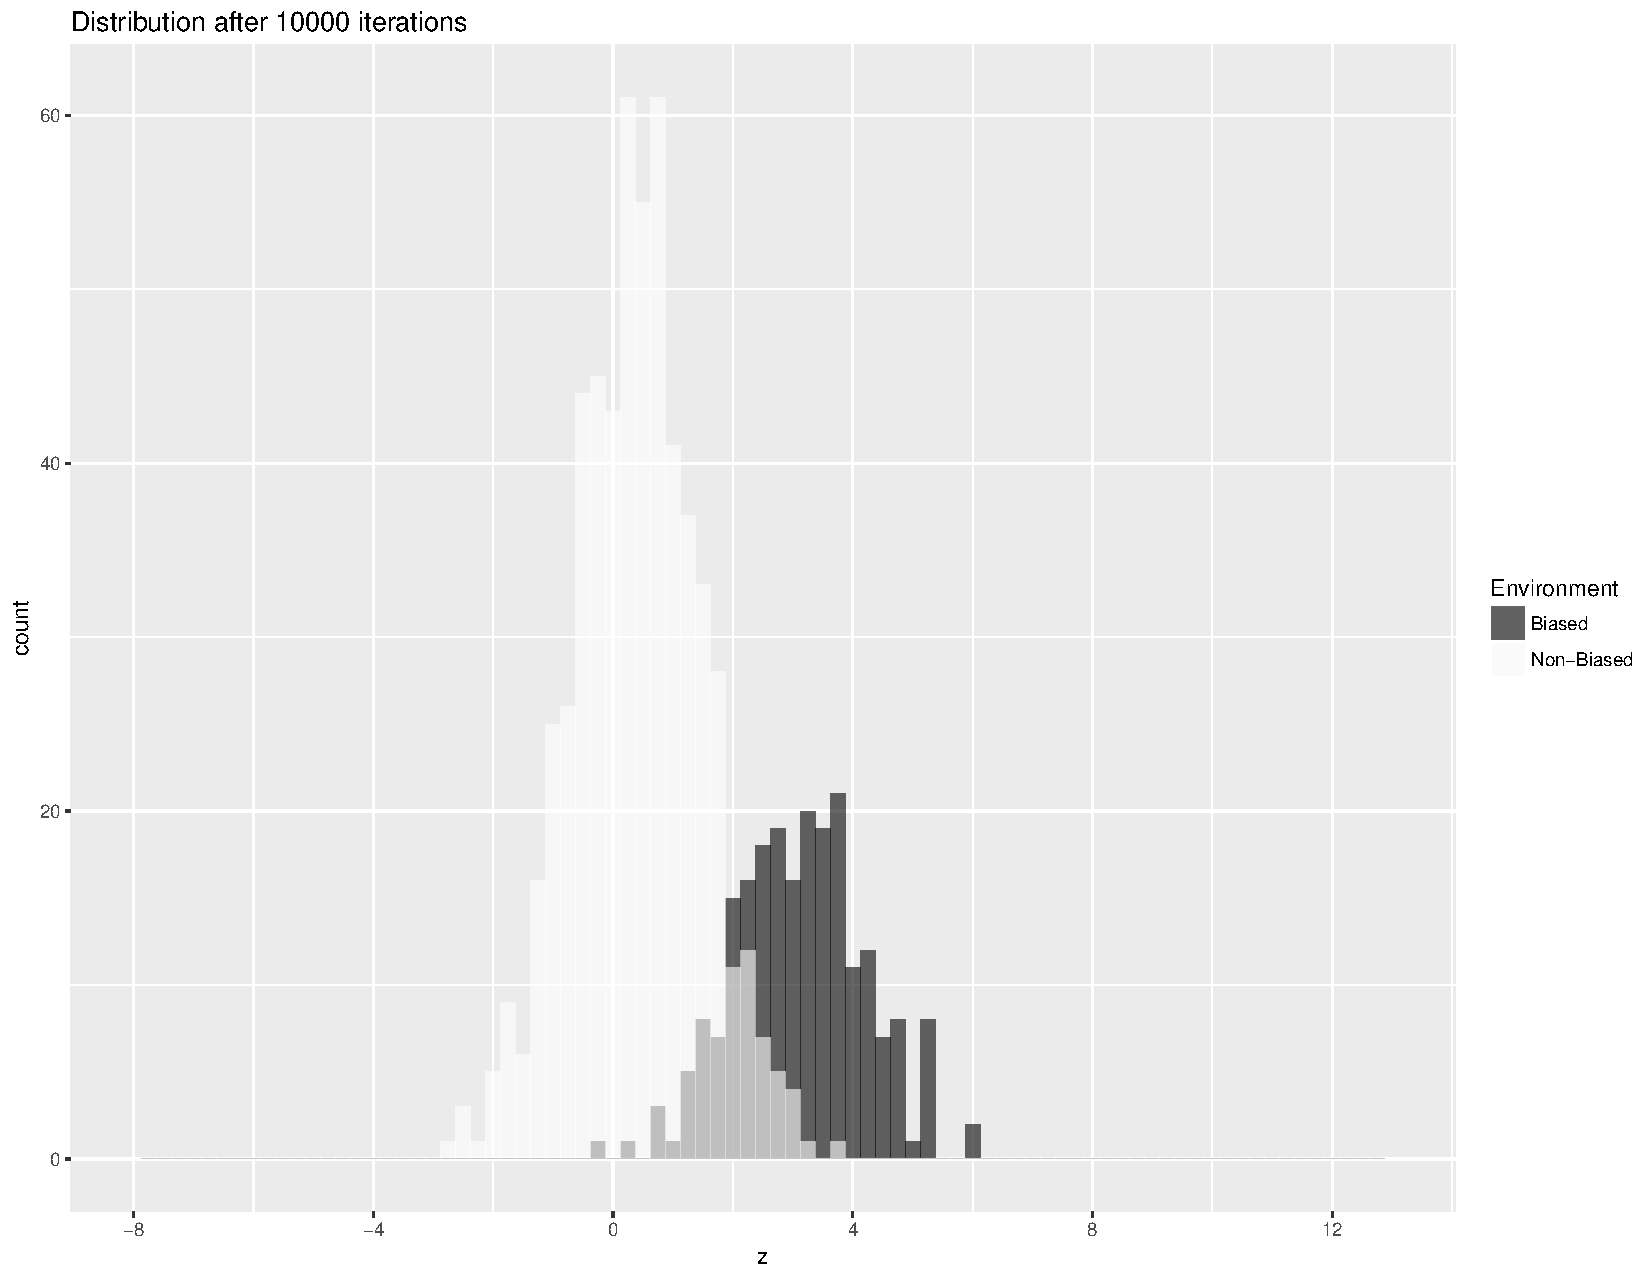
\includegraphics[scale=0.3]{figures/BaselineModel10000iter.pdf}\caption{\label{fig:Model2:LengtheningProcess}Soft-Target Model with increasing
bias function. White: tokens produced
in non-biasing contexts. Black: tokens produced in biasing contexts.
z-normed \emph{x} dimension. Observation occurs after 10,000
model cycles.}
\end{figure}

For positive \emph{x}, the difference between (\ref{eq:Lengthening Force})
and (\ref{eq:Inertia Force}) is effectively between a monotonically
increasing function with an optimum at 0, and a non-monotonic function
with an optimum at \emph{N}. Theoretically speaking, however, the
former expresses a \textsc{process}, while the latter expresses a
\textsc{state} (cf. \citealt{Hyman1975}). \textsc{process }will be
taken to refer to what would be considered an allophonic rule in generative
phonology, and to which the term ``lengthening'' (or ``shortening'') can
properly apply. At the segment level (\emph{S}), the general process
model instantiates the following linguistic relationship: $/S/\rightarrow[S{}^{B}]/$\emph{\_\_B}\textsc{,
}where\emph{ B} stands for the biasing context, and $[S^{B}]$ stands
for the allophonic variant that occurs in that context. Using the
same notation, a \noun{state} model instantiates the following relationship:
$/S^{B}/\rightarrow[S{}^{B}]$ in context \emph{B}. This indicates
that $S^{B}$ is stored, or underlying, rather than generated. A given
\textsc{state} could consist of ``long'', or ``lengthened'', tokens but
does not properly involve ``lengthening''. 

\section{\label{sec:Model-Interpretation}Model space}

The original lengthening model in \sectref{subsec:Phrase-Final Lengthening}
is a \textsc{process} model. As we saw previously, a \textsc{process}
model that lacks a production target is unbounded, producing no stable
outcomes. As will be shown in Section \ref{subsec:Model-B:-Lengthening},
adding a soft target to this model will result in stable outcomes
for a certain range of parameter values. The analogous \textsc{state}
model can be created by implementing the bias term itself as a soft
target, as in (\ref{eq:Length Attractor}) (cf. \citealt{soskuthy2013phonetic}). 
\begin{equation}
L(x_{i})=\alpha(L-x_{i})\label{eq:Length Attractor}
\end{equation}
This model, with one target for non-biased tokens and one for biased
tokens, can also be shown to produce stable outcomes. The no-target
\noun{process} model, the soft-target \noun{process} model, and the
\noun{state} model, however, differ with respect to their theoretical
consistency and thus linguistic interpretability. 

Model 2, from \sectref{subsec:Phrase-Final Lengthening}, re-labelled
as Model A in Table~\ref{tab: Model Comparison-1}, is a linguistically
interpretable model. There is a single category from which tokens
are selected at random, either to be produced in biasing contexts,
in which case they are lengthened, or to be produced in non-biasing
contexts, in which case they are unchanged. Model B, with a soft target
at the location of the non-biased, underlying category, is also consistent.
All tokens feel a pull towards this underlying target, but those that
happen to be produced in a biasing context are also subject to a force
that lengthens them during production. Model C, however, the \textsc{state}
model, is not theoretically consistent. 

\begin{table}[h]\footnotesize
\caption{Single-Category Model Space\label{tab: Model Comparison-1}}
\begin{tabular}{ccccccc}
\lsptoprule
 & \multicolumn{2}{c}{} & \multicolumn{2}{c}{} & Stable & Consistent\tabularnewline
\midrule
A & \textsc{Process} & $\alpha(1+x)$ & No Target & – & N & Y\tabularnewline
B & \textsc{Process} & $\alpha(1+x)$ & Target & $\beta(N-x)$ & (Y) & Y\tabularnewline
C & \textsc{State} & $\alpha(L-x)$ & Target & $\beta(N-x)$ & Y & N\tabularnewline
\lspbottomrule
\end{tabular}
\end{table}

In Model C, all tokens have a target at \emph{N}, but tokens produced
in a biasing context have an additional, conflicting target at \emph{L}.
Because there is only a single category in Model C, biased tokens
are generated from the same pool as non-biased tokens, therefore the
second target, \emph{L}, exists without an underlying category with
which that target can be associated. With the distribution initialized
at \emph{N}, the effect is for biased tokens to be moved an arbitrarily
small distance, $\alpha(L-x)$, towards that second target during
production.\footnote{As a \noun{process}, incrementality has a straightforward interpretation:
a given token is shifted, or lengthened, by a fixed proportion of
its current length. But in a \textsc{state} model, in which all tokens
are initialized at one target, it is not clear what mechanism would
shift certain tokens only a small amount towards another target. Although,
superficially, this effect is similar to that of the entrenchment
force, $\varepsilon(\overline{x}-x)$, which pushes the tokens of
a given category closer together, they are different in important
ways. The use of the category mean in the entrenchment function stands
in for the sum of the forces that act between individual tokens, maintaining
category cohesion (the same effect can be achieved by averaging over
multiple tokens in production (e.g. \citealt{Pierrehumbert2000,Wedela})).
The soft target, or inertia force, on the other hand, references a
fixed target location that is specified independently of the current
distribution. } Of the three models, only Model B is both stable (bounded) and
theoretically consistent. 

Model C, however, can be made theoretically consistent by introducing
a second level of representations. If the parent category can be split
into two sub-categories, then each target can be associated with a
different sub-category. This is Model G in Table~\ref{tab: Model Comparison},
which is the 2-level model analog of Table~\ref{tab: Model Comparison-1}.
The remaining models in this table are all theoretically problematic
in different ways. Model D is the two sub-category counterpart of
Model B. While Model B is theoretically consistent, the introduction
of a separate sub-category for biased tokens in Model D creates a
representational paradox: a category with no target, to which lengthening
continuously applies. Model D is also unbounded. Model E re-creates
the two-target paradox of Model C. Finally, F is the hybrid \noun{process}+\emph{state}
model.\footnote{If double specifications are possible (e.g. \textsc{process} + \textsc{state}),
then the total set of possible models includes the Single-Category
\textsc{process}+\textsc{state} model, and the set of non-biased No-Target
models, among others. However, these other models all contain a superset
of the representational inconsistencies already described, and therefore
are not included.}

\begin{table}[h]\footnotesize
\caption{2-Level Model Space\label{tab: Model Comparison}}
\begin{tabular}{ccccccc}
\lsptoprule
 & \multicolumn{2}{c}{biased} & \multicolumn{2}{c}{non-biased} & Stable & Consistent\tabularnewline\midrule
D & \textsc{Process} & $\alpha(1+x)$ & Target & $\beta(N-x)$ & N & N\tabularnewline
E & \textsc{2-State} & $\beta(N-x)$; $\alpha(L-x)$ & Target & $\beta(N-x)$ & Y & N\tabularnewline
F & \textsc{Process+ State} & $\alpha(1+x)$; $\alpha(L-x)$ & Target & $\beta(N-x)$ & Y & N\tabularnewline
G & \textsc{State} & $\alpha(L-x)$ & Target & $\beta(N-x)$ & Y & Y\tabularnewline
\lspbottomrule
\end{tabular}
\end{table}

Only two viable candidates emerge from the full set of model: a pure
\textsc{process} model with a single target, (B), and a pure \textsc{state}
model (G). In general terms, these results show us that \textsc{process}
and \textsc{state} models are incompatible with one another. If biased
tokens have a separate representational status, this implies that
only tokens from this sub-category should be chosen to be produced
in biased contexts. Furthermore, since the biased sub-category has
a target at \emph{L}, those tokens will already be appropriately longer
than their non-biased counterparts (with a target at \emph{N}). Therefore,
there is no motivation for lengthening them further. Effectively,
this would be equivalent to a phonological rule of the form:
\begin{covexamples}
\item \label{Process-+-State:}Process + State: $/S^{B}/\rightarrow[S{}^{B^{B}}]/$\emph{\_\_B}
\end{covexamples}
Although (\ref{Process-+-State:}) is linguistically ill-formed, it
is equivalent to the feedback loop at the heart of the basic exemplar
model.\footnote{It should be noted that, as far as I am aware, no one has actually
proposed the context-dependent exemplar models in \chapref{ch:The-Exemplar-Model}.
They are what I take to be the logical extension of the context-free
exemplar model of \citet{Pierrehumbert2000}.} Cumulativity of small differences is only possible if the bias effects
in production (contextually determined allophony) are stored (\noun{state}),
rather than being stripped away during perception. Storage of allophonic
detail implies that the biasing context itself is discarded, or at
least not used to recover the underlying form. In production, however,
the \textsc{process} model requires knowledge of the context that
triggers biasing. In other words, the allophonic rule is available
in production, but not in perception.\footnote{The alternative is that both the unnormalized surface forms and their
production context are stored, or incorporated into the category label
in some way. Even if so, it is still not clear why an allophonic rule
would continue to apply. Furthermore, if prior specification of complex
sub-structure is required (and, in the limit, a unique category for
every token), the exemplar framework does not seem to offer much, if
anything, in terms of explanatory power. }

Another way to characterize this theoretical incompatibility is that
a \textsc{process} model implies that normalization takes place, while
a \textsc{state} model implies that it does not. Thus, inconsistency
results when either the production or perception stage of a given
model assumes normalization, while the other doesn't. In the Pure
Process Model (B), all tokens are drawn from the same distribution
in production, with a target, or underlying specification, at \emph{N}.
Lengthening applies as an allophonic rule, but in perception all tokens
are drawn back to the same underlying target at \emph{N}, whether
they are lengthened or not. Thus, the inertial force acts to partially
normalize the effect of lengthening. Complete normalization (fixed
target) would prevent change entirely. In the Pure State Model (G),
on the other hand, normalization fails to occur in the sense that
``lengthened'' tokens are assigned to their own sub-category, and no
allophonic rules apply. Again, the \textsc{state} aspect is only partial.
The fact that these are sub-categories rather than completely independent
categories introduces a connection between the biased and non-biased
tokens which implies that the relationship between them is known,
and therefore that the allophonic transformation is known. Two entirely
independent categories would preclude change entirely. 

\section{\label{sec:Model-Behavior}Consistent and convergent models of sound change}

This section is devoted to an exhaustive analysis of the end states
of the two theoretically consistent and bounded models: the Pure Process
Model (B), and the Pure State Model (G). These results will be provided
in the form of two parameters: the category means along the dimension
\emph{x}, and the difference between the means of the biased and non-biased
sub-distributions. Because it is not possible to guarantee that simulations
will fully sample the space of possible outcomes, stable states will
be explicitly derived as a function of model parameters. The derivation
will be given in abbreviated terms in the text, with the full details
provided in the appendices. Following \citet{soskuthy2013phonetic,Soskuthy2015},
the percentage of tokens produced in a biasing context (bias proportion)
will act as the independent variable. The term “attractor” will
also be adopted in reference to a soft target, in order to facilitate
comparison to that work. 

\subsection{\label{subsec:Lengthening-as-State}State Model: Sub-categories}

The Pure State Model contains one target for biased tokens, and a
distinct target for non-biased tokens. Figure \ref{fig:Model G} provides
an illustration of the forces acting at some model time \emph{t},
on exemplar categories modeled as normal functions. As will be shown
below, the means of both sub-categories can be guaranteed to lie somewhere
between the two targets at \emph{N} and \emph{L}. Each sub-category
is subject to the inertia associated with its own target, acting to
pull the two apart. Membership in a superset category is implemented
via the entrenchment force, which pulls both in the direction of the
global mean, and thus towards one another.\footnote{\citet{soskuthy2013phonetic} links sub-categories by applying phonetic
biasing probabilistically to both, but with the biased sub-category
more strongly weighted. } In this illustration, the relative number of tokens produced in
biasing versus non-biasing contexts is represented by the heights
of the normal curves. Because the proportion of biasing contexts is
less than 50\% in this example, the global mean (indicated by the
dashed line) is closer to the mean of the non-biased distribution. 

\begin{figure}[H]
\begin{centering}
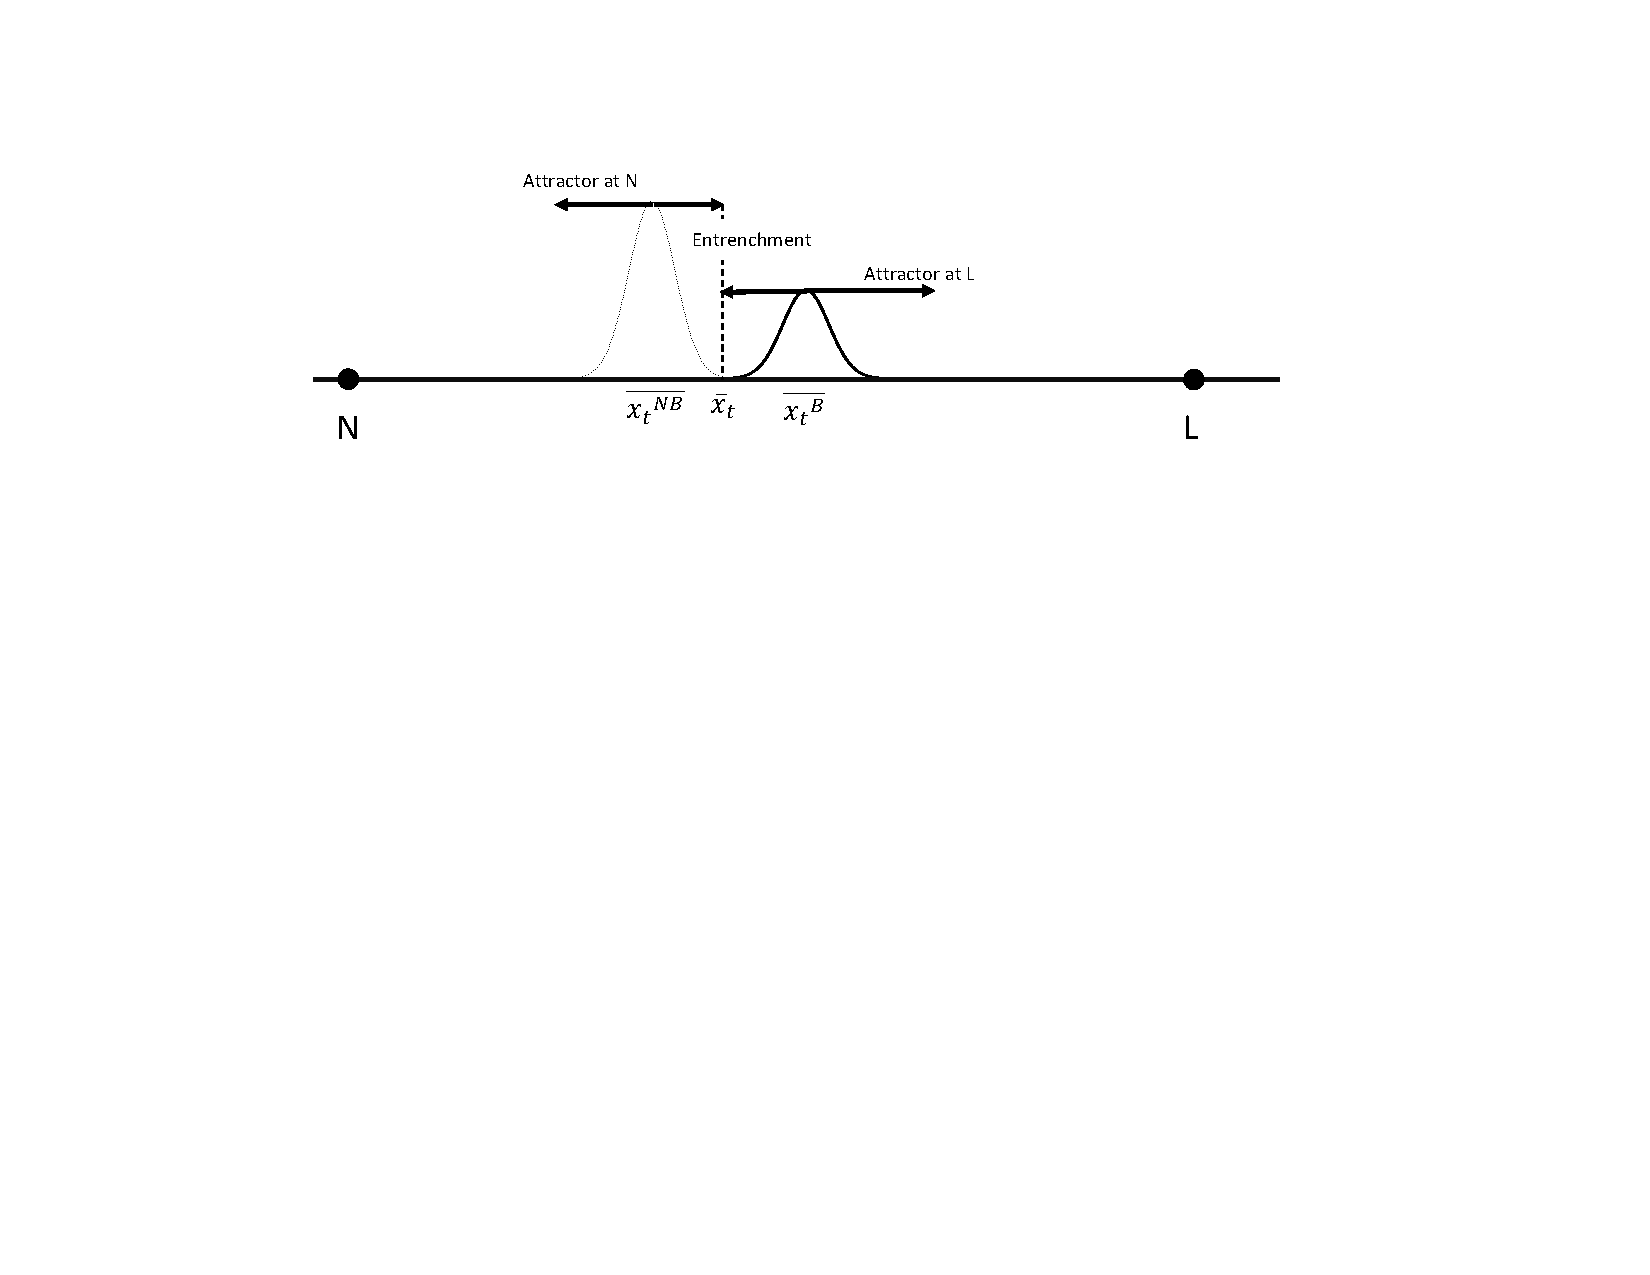
\includegraphics[width=.75\textwidth]{figures/Model6Behavior.pdf}\caption{\label{fig:Model G}Schematic of forces for Pure State Model}
\par\end{centering}
\end{figure}

The equations for each of the model forces have been given previously,
but are repeated here for ease of reference: (\ref{eq:Entrenchment-2})
Entrenchment, (\ref{eq:Inertia-2}) Inertia (attractor) at \emph{N},
and (\ref{eq:Length Attractor-2}) Inertia (attractor) at\emph{ L}.
A small random error term is also included in all models. 
\begin{equation}
E(x_{i})=\epsilon(\overline{x}-x_{i})\label{eq:Entrenchment-2}
\end{equation}
\begin{equation}
I(x_{i})=\beta(N-x_{i})\label{eq:Inertia-2}
\end{equation}
\begin{equation}
L(x_{i})=\alpha(L-x_{i})\label{eq:Length Attractor-2}
\end{equation}
In order to estimate the behavior of this model under various conditions
we will make the simplifying assumption that each sub-category is
specified by a normal curve with variable mean, but fixed standard
deviation. This allows us to use the mean of each sub-category as
a proxy for its global behavior. To determine the stable model outputs,
we use the fact that forces must balance at this equilibrium point,
meaning that no further changes occur in the location of the means.
Therefore, the sum of all forces is set to zero. $\overline{x_{E}}$
is defined as the location of the global mean at equilibrium, while
$\overline{x_{E}^{B}}$ and $\overline{x_{E}^{NB}}$ are the equilibrium
means of the biased and non-biased sub-categories, respectively. 

The first step is to prove that there is no way for the mean of either
sub-category (and therefore, the global mean) to have a value less
than \emph{N}, or greater than \emph{L}. This follows from the mathematical
form of the inertial, or attractor, forces. For values greater than
the attractor location, the force is leftward, but for values smaller
than the attractor location, the force is rightward, thus always acting
to push the distribution precisely to the attractor location. If the
sub-categories were completely independent (no global entrenchment),
then they would always stabilize at their respective attractor locations.
Entrenchment allows the sub-categories to be perturbed from their
attractors, but only in the direction of the other sub-category. Thus,
we can be confident that they will end up at equilibrium somewhere
between \emph{N} and \emph{L}. The exact location will depend on the
parameters $\alpha$ (the strength of the attractor at \emph{L}),
$\beta$ (the strength of the attractor at \emph{N}), $\varepsilon$
(the strength of the entrenchment force), and $p$ (the bias proportion:
the percentage of the category consisting of biased tokens; in other
words, the percentage of tokens produced in a biasing context). 

The equilibrium location for the non-biased sub-category is determined
by the point at which global entrenchment (\ref{eq:Entrenchment})
is perfectly balanced by the attractor at \emph{N} (\ref{eq:Inertia Force}).
Using the equilibrium location of the mean to stand in for the entire
sub-category: \[\beta\left(N-\overline{x_{E}^{NB}}\right)+\varepsilon\left(\overline{x_{E}}-\overline{x_{E}^{NB}}\right)=0\text{.}\]
Therefore, \[\beta\left(\overline{x_{E}^{NB}}-N\right)=\varepsilon\left(\overline{x_{E}}-\overline{x_{E}^{NB}}\right)\text{.}\]
For the biased distribution, it is the attractor at \emph{L} (\ref{eq:Length Attractor})
that will be balanced by global entrenchment (\ref{eq:Entrenchment}):
$\alpha(\overline{x_{E}^{B}}-L)=\varepsilon(\overline{x_{E}}-\overline{x_{E}^{B}})$.
In order to solve for the three quantities, $\overline{x_{E}^{B}}$,
$\overline{x_{E}^{NB}}$ , and $\overline{x_{E}}$ , we need a third
equation linking them. This is given by the equation that expresses
the global mean as a weighted average of the two sub-category means.
\begin{equation}
\overline{x_{E}}=(1-p)\overline{x_{E}^{NB}}+p\overline{x_{E}^{B}}\label{eq:weighted mean}
\end{equation}
We can now solve for each of the quantities in turn by substitution.
Appendix C shows the full derivation, and demonstrates that the global
mean at equilibrium, $\overline{x_{E}}$ , can be expressed in the
following terms:
\begin{equation}
\overline{x_{E}}=\frac{(1-p)\beta N(\alpha+\varepsilon)+p\alpha L(\beta+\varepsilon)}{(\beta+\varepsilon)(\alpha+\varepsilon)-(\alpha+\varepsilon)(1-p)\varepsilon-(\beta+\varepsilon)p\varepsilon}\label{eq: sub-dist}
\end{equation}
as a function of the set of model parameters ($\alpha,\beta,N,L,p$),
the location of the global mean at equilibrium. The other quantity
of interest is the distance between the sub-category means, which
can be expressed as a function of $\overline{x_{E}}$ :
\begin{equation}
\Delta\overline{x_{E}}\equiv\overline{x_{E}^{B}}-\overline{x_{E}^{NB}}=\frac{\alpha L+\varepsilon\overline{x_{E}}}{\alpha+\varepsilon}-\frac{\beta N+\varepsilon\overline{x_{E}}}{\beta+\varepsilon}\label{eq:State Model-sep}
\end{equation}
Keeping all other variables constant, we can now derive the behavior
of these two quantities as a function of the bias proportion, \emph{p}. 

The change in $\overline{x_{E}}$ that results from a change in \emph{p}
is given by taking the partial derivative of Eq. (\ref{eq: sub-dist}).
This turns out to be somewhat unwieldy to calculate in general form.
In the special case when all forces have the same strength ($\alpha=\beta=\varepsilon$),
we can show that Eq. (\ref{eq: sub-dist}) reduces to $\overline{x_{E}}=N+p(L-N)$.
Therefore, the global category mean is a positive linear function
of \emph{p}, and the change in the location of that mean is constant:
${\partial\overline{x_{E}}}/{\partial p}=L-N$. 

For other cases, it's possible to determine the general behavior of
${\partial\overline{x_{E}}}/{\partial p}$ even without an exact
solution. Assume that the equilibrium state for a given $p=p_{j}$
has already been determined. Now increase \emph{p} to $p_{k}$. Eq.
(\ref{eq:weighted mean}) entails that if $p_{k}>p_{j}$ (an increase
in bias proportion), then the global mean will shift closer to the
biased sub-category. Because the strength of the entrenchment force
depends on the distance from the global mean, this shift will, in
turn, cause the entrenchment force on the non-biased sub-category
to increase. Because the attractor at \emph{N} and the entrenchment
force are taken to be perfectly balanced at $p=p_{j}$, an increase
in the latter will result in a shift of the non-biased sub-category
toward the biased one. At the same time, the entrenchment force on
the biased sub-category will decrease commensurately. In this case,
a decrease in the entrenchment force causes the balance to shift in
favor of the attractor at \emph{L}, meaning the biased sub-category
will also shift in the rightward direction. Because the sub-categories
shift in the same direction, the equilibrium point for the global
mean is also guaranteed to shift in that direction, and thus to increase
as \emph{p} increases: ${\partial\overline{x_{E}}}/{\partial p}>0$. 

In the special case where $\alpha=\beta=\varepsilon$, we can use
the result that ${\partial\overline{x_{E}}}/{\partial p}=L-N$,
and determine that ${\partial\Delta\overline{x_{E}}}/{\partial p}=0$.
Therefore, the distance between the two sub-categories remains constant
in this case. The general form of the partial derivative of (\ref{eq:State Model-sep})
with respect to \emph{p}, ${\partial\Delta\overline{x_{E}}}/{\partial p}$,
can be written as a function of the partial derivative of $\overline{x_{E}}$
with respect to \emph{p} (${\partial\overline{x_{E}}}/{\partial p}$):
\begin{equation}
\frac{\partial\Delta\overline{x_{E}}}{\partial p}=\frac{\partial\overline{x_{E}}}{\partial p}\varepsilon\left[\frac{1}{\alpha+\varepsilon}-\frac{1}{\beta+\varepsilon}\right]\label{eq: Model G: dsep/dp}
\end{equation}
Since we know that ${\partial\overline{x_{E}}}/{\partial p}$
is always positive, the sign of ${\partial\Delta\overline{x_{E}}}/{\partial p}$
is determined by the sign of ${1}/({\alpha+\varepsilon})-{1}/({\beta+\varepsilon})$.
The sign of ${1}/({\alpha+\varepsilon})-{1}/({\beta+\varepsilon})$
is determined by the relative sizes of the quantities $\alpha+\varepsilon$,
and $\beta+\varepsilon$. Therefore, if $\alpha>\beta$ then ${\partial\Delta\overline{x_{E}}}/{\partial p}<0$;
and if $\alpha>\beta$ , then ${\partial\Delta\overline{x_{E}}}/{\partial p}<0$.

\subsection{\label{subsec:Model-B:-Lengthening}Process Model: Single category}

The Pure Process Model contains a single category, and a single target
for that category. Tokens are selected at random, with probability
\emph{p,} to be produced in the biasing context. This model is identical
to the Soft Target Model described in Section \ref{subsec:Soft-Targets}
(\figref{fig:Model2:LengtheningProcess}). It will be shown in this
section that the Process Model is only stable for certain parameter
values. The behavior of the global mean, and the average separation
between biased and non-biased productions, will be derived as before.
The same simplifying assumption that the category can be approximated
as a normal distribution with fixed variance will also be made. However,
it should be noted that this assumption is less justified for the
one-category model due to the fact that biased and non-biased variants
will separate, creating a lumpier distribution, and likely an increase
in variance.

The derivational steps in this analysis are given graphically in \figref{fig:Derivation}.
Panel 1 is a snapshot of the model at some
time, \emph{$t$}, when the global mean is located at location $\overline{x_{t}}$
along \emph{x}. Both biased and non-biased tokens are sampled from
this distribution, at different rates. This relationship is indicated
by the darker normal curve (subset of tokens subjected to bias during
production) within the lighter one (subset of tokens non-biased during
production). 

\begin{figure}[h]
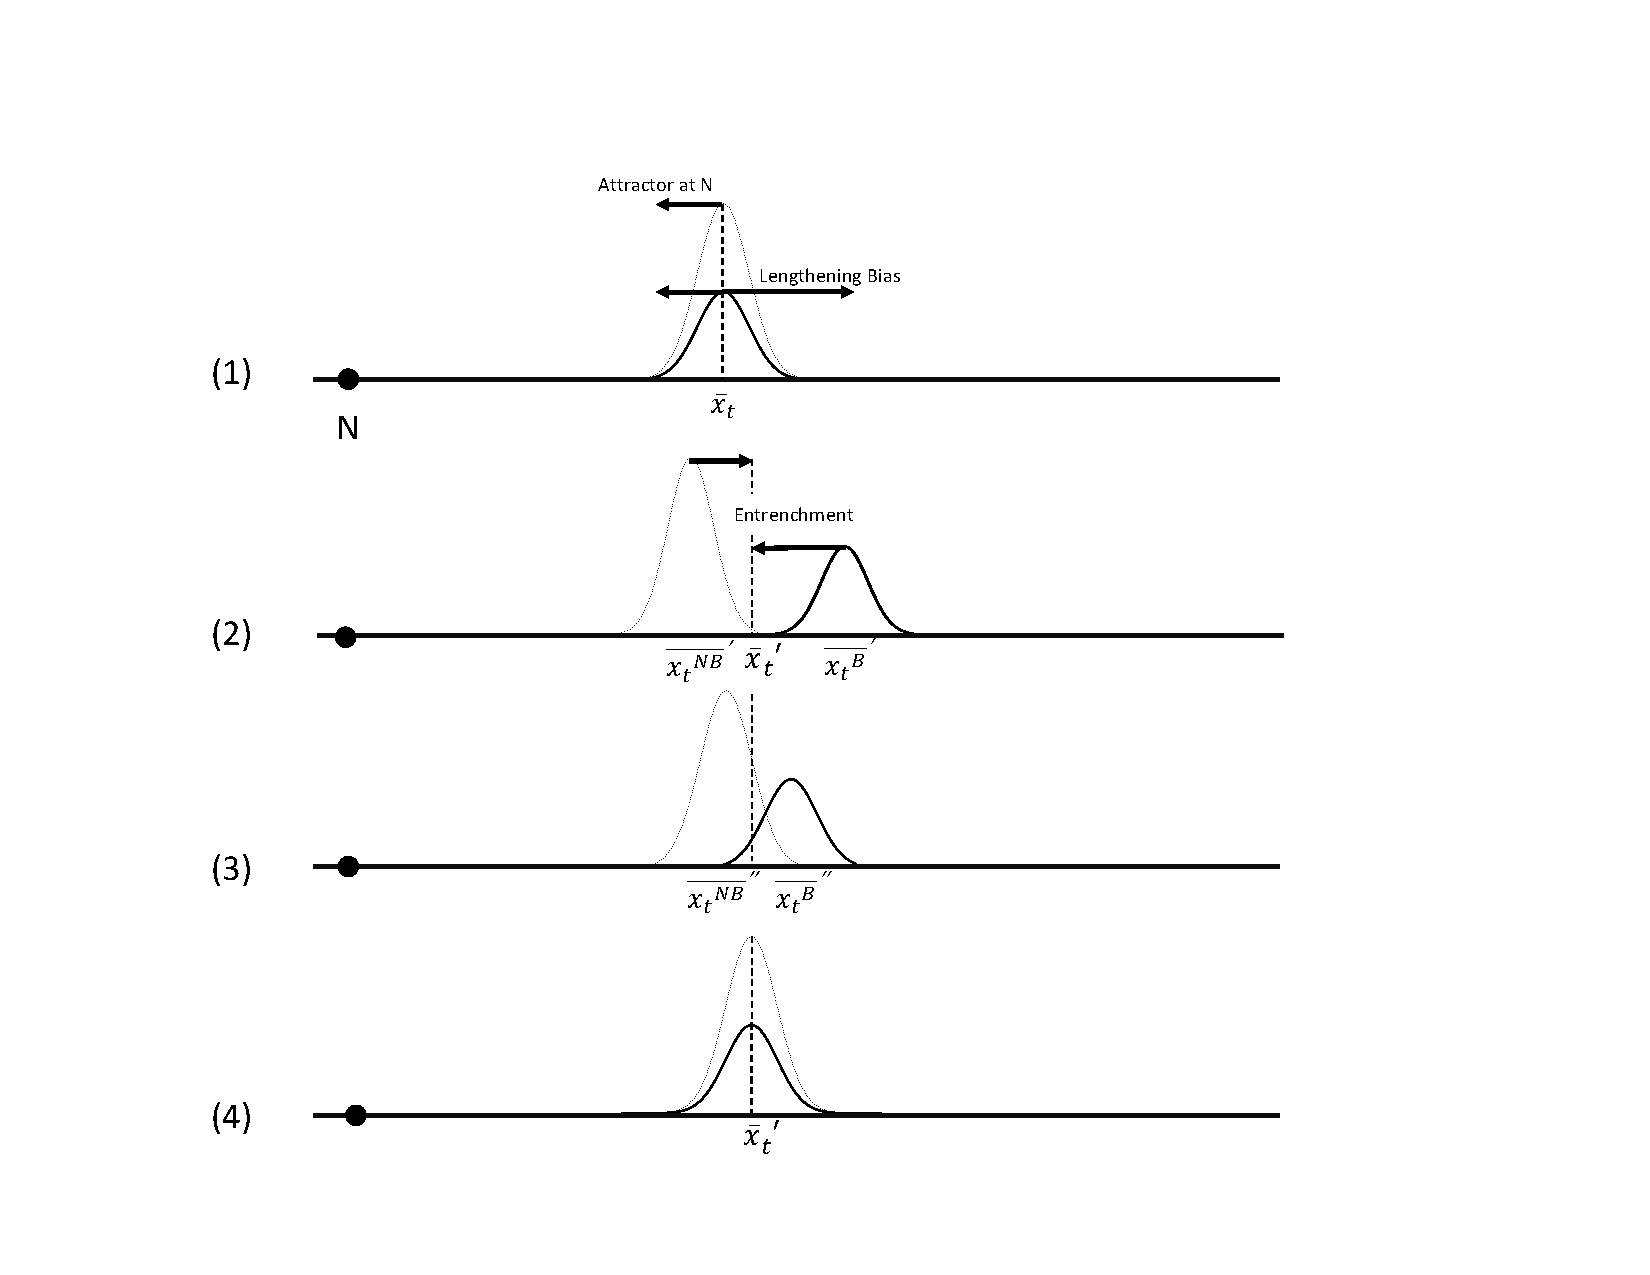
\includegraphics[width=0.50\textwidth]{figures/Model1Behavior.pdf}\caption{\label{fig:Derivation}Schematic of forces for \noun{process} model}
\end{figure}

The production value of any token at any time \emph{t} can be calculated,
as long as its current value, and the category mean, are known. All
tokens are subject to the attractor at \emph{N}. And all tokens are
subject to the entrenchment force acting to pull them closer to the
current category mean (which will be greater than, or equal to, \emph{N}).
Additionally, a proportion \emph{p} of randomly selected tokens undergo
a lengthening process, moving away from the rest of the distribution
during production.

Panels 2--4 of \figref{fig:Derivation} take us sequentially through
the application of forces. Panel 2 isolates the effect of applying
the attractor and lengthening forces. The attractor affects all tokens
equally, because all tokens are equally far from \emph{N} on average.
Lengthening, applied only to a subset of tokens, splits the distribution
apart. Before entrenchment applies, the mean values for the observed
productions ($\overline{x_{t}^{B}}^{\prime}$, mean of biased productions
in Panel 2; $\overline{x_{t}^{NB}}^{\prime}$, mean of non-biased productions
in Panel 2), can each be given as a function of the global mean at
time $t$, $\overline{x_{t}}$:
\begin{equation}
\overline{x_{t}^{B}}^{\prime}=\overline{x_{t}}(1+\alpha)+\beta(N-\overline{x_{t}})\label{eq:Biased}
\end{equation}
\begin{equation}
\overline{x_{t}^{NB}}^{\prime}=\overline{x_{t}}+\beta(N-\overline{x_{t}})\label{eq:Non-biased}
\end{equation}
Applying entrenchment does not affect the global mean, only the absolute
locations of the sub-distribution means, and their separation. Therefore,
the mean in Panel 3 is identical to the mean from Panel 2. This mean
($\overline{x_{t}}^{\prime}$) is given by the weighted average of the
means of the observed production variants: 
\begin{equation}
\overline{x_{t}}^{\prime}=(1-p)\overline{x_{t}^{NB}}^{\prime}+p\overline{x_{t}^{B}}^{\prime}\label{eq: G weighted mean}
\end{equation}
Equilibrium is achieved when continued iterations fail to change the
locations of the means. This means that they should be unaffected
by successive iterations of biasing. $\overline{x_{E}}^{\prime}=\overline{x_{E}}$
, $\overline{x^{B}}^{\prime}=\overline{x^{B}}$, and $\overline{x^{NB}}^{\prime}=\overline{x^{NB}}$.
Therefore, 
\begin{equation}
\overline{x_{E}}=(1-p)\overline{x_{E}^{NB}}^{\prime}+p\overline{x_{E}^{B}}^{\prime}\label{eq:equilbrium 1}
\end{equation}
and from Eq. (\ref{eq:Biased}) and (\ref{eq:Non-biased}), 
\begin{equation}
\overline{x_{E}}=(1-p)\{\overline{x_{E}}+\beta(N-\overline{x_{E}})\}+p\{\overline{x_{E}}(1+\alpha)+\beta(N-\overline{x_{E}})\}\label{eq:equilbrium 2}
\end{equation}
Solving for $\overline{x_{E}}$ gives
\begin{equation}
\overline{x_{E}}=\frac{\beta N}{\beta-p\alpha}\label{eq: lengthening process}
\end{equation}
See Appendix \ref{chap:Appendix D} for the full derivation. 

The behavior of the global mean as a function of \emph{p} will depend
on which region of parameter space we are in: $p\alpha<\beta$, or
$p\alpha>\beta$. For $p\alpha<\beta$, the denominator in (\ref{eq: lengthening process})
is positive. Therefore, as \emph{p} increases (but $p\alpha$ stays
smaller than $\beta$), the denominator decreases, and the global
mean increases (${\partial\overline{x_{E}}}/{\partial p}>0$).
In the limit, as $p\alpha$ goes to $\beta$, the equilibrium mean
goes to infinity, and lengthening is unbounded. For $p\alpha>\beta$
, the denominator is negative, which also means that the mean is negative,
and the only equilibrium point is negative. Since negative duration
values aren't possible, there is no well-defined equilibrium in the
range in which $p\alpha>\beta$. The \noun{process} model is thus
only stable if the lengthening strength ($\alpha$) is not too great,
and the percentage of biasing contexts ($p$) is not too large, relative
to the attractor strength ($\beta$).

To calculate the second quantity of interest, the dependence of sub-distribution
separation on \emph{p,} the effect of entrenchment must be included.
Entrenchment acts to bring all tokens back towards the global mean
by an amount proportional to their distance from that mean (Panel
3 of \figref{fig:Derivation}): 
\begin{equation}
\overline{x^{B}}^{\prime\prime}=\overline{x^{B}}^{\prime}+\varepsilon\left(\overline{x}^{\prime}-\overline{x^{B}}^{\prime}\right)\label{eq:Panel 3 biased}
\end{equation}
\begin{equation}
\overline{x^{NB}}^{\prime\prime}=\overline{x^{NB}}^{\prime}+\varepsilon\left(\overline{x}^{\prime}-\overline{x^{NB}}^{\prime}\right)\label{eq:Panel 3 unbiased}
\end{equation}
The separation between the two production variants after entrenchment
applies ($\varDelta\overline{x}^{\prime\prime}$) can be determined
by taking the difference between Equations (\ref{eq:Panel 3 biased})
and (\ref{eq:Panel 3 unbiased}): 
\begin{equation}
\varDelta\overline{x}^{\prime\prime}\equiv\overline{x^{B}}^{\prime\prime}-\overline{x^{NB}}^{\prime\prime}=\left(1-\varepsilon\right)\left(\overline{x^{B}}^{\prime}-\overline{x^{NB}}^{\prime}\right)
\end{equation}
The final separation depends only on the separation prior to the application
of entrenchment ($\varDelta\overline{x}^{\prime}$ in Panel 2), and
the strength of the entrenchment term, $\varepsilon$. Because the
sub-distributions only exist at production, no cumulativity in separation
is possible (see Panel 4). Therefore, at all times \emph{t}, the separation
in Panel 2, prior to entrenchment, will always be given by the lengthening
factor: $\alpha\overline{x_{t}}$. Therefore, at equilibrium, when
$\overline{x_{t}}=\overline{x_{E}}$, the average distance between
the two production sub-distributions is given by
\begin{equation}
\varDelta\overline{x_{E}}=(1-\epsilon)(\alpha\overline{x_{E}}).\label{eq:Cat Sep}
\end{equation}
In the stable parameter range ($p\alpha>\beta$), where $\overline{x_{E}}$
increases as \emph{p} increases, the separation of the sub-distributions
also increases, but more slowly, by a factor of $(1-\epsilon)\alpha$.

\section{\label{sec:Actuation}Change between stable states}

Most work in the exemplar framework models either change or stability,
but not both. That is to say, only one stable state is possible, and
the model either starts in that state, in which case it remains there
for all time, or inevitably arrives in that state from any other starting
conditions. In \citet{Garrett2013} there are two different modes
of processing,\footnote{These are likened to “speech” and “non-speech” processing
modes (\citealt{liberman1967perception}); individual speakers may
switch between the two modes, or different speakers may operate consistently
in one or the other mode (e.g. \citealt{yu2013socio}). } resulting in essentially two different models: one in which normalization
occurs, which is stable, and one in which normalization is “turned
off”, leading to change (the latter model is not implemented, but
would lead to unbounded shift without an additional mechanism). \citet{Kirby2014}
is similar in that two different outcomes are possible, one for a
``misparsing'' mode, and one for accurate parsing (in the ``misparsing''
mode, merger is prevented by a stage of hypothesis selection in which
a Bayesian learner updates phonetic cue weights so as to optimize
categorization accuracy). 

“Agent-based” models (not all implemented using exemplar representations)
use the interaction among one or more groups of speakers to be the
driving mechanism, either of the evolution of language itself, or
of the evolution of pre-existing variants (which may be parameters,
or entire grammars). Systems are taken to be stable within individual
speakers, that is, without bias. Thus there is no mechanism via which
a truly novel form can arise, only ways in which an existing distribution
can evolve within a heterogeneous population (\citealt{Niyogi1997,Boer2000,nowak2001evolution,Steels2005,baxter2006utterance,oudeyer2006self,fagyal2010centers,stanford2013revisiting,pierrehumbert2014model}).
Models that rely on simple ``self-organizing'' principles, such as random
selection, or mis-classification, are usually designed to demonstrate
that a single optimal state will be reached from any starting position
(\citealp{Wedela,ettlinger2007exemplar,Wedel2006,Blevins2009,DBLP:journals/corr/Tupper14a,wedel2017category}).
Some additional mechanism would be needed to change such systems further.
Effectively, actuation is achieved either through speaker contact
(in which adoption of already existing variants may occur), or by
initializing the model in an unstable state. 

As far as I am aware, \citet{soskuthy2013phonetic} and \citet{Soskuthy2015}
are unique in the literature in that they capture both change and
stability within a single model. Actuation occurs via a completely
speaker-internal mechanism that is an integral component of the model:
allophone frequency. Model 1 in \sectref{subsec:Model-1:-Context-Free}
was an instantiation of frequency of use as an instigator of change,
in the successive reduction of highly frequent words. In that model,
frequency was a fixed property of a given word type. But changes in
word frequency, as well as in the relative proportion of contextual
variants, are possible for independent reasons. Words go in and out
of style, and the frequency of use of any given word is expected to
change over time. In turn, changes in frequency at the word level
also affect the frequency of occurrence of the phonemes that make
up the word. A change in allophone frequency could also result if
the words affected happened to contain the same allophonic environment. 

The model of vowel lengthening in \citet{soskuthy2013phonetic} was
the basis for the gradient context-dependent model first introduced
in \sectref{sec:Context-Dependent-Iterativity}. This model was
gradually developed, first into a set of possible models implementing
at least one soft target, then into a subset of those that were both
stable and theoretically consistent. The remaining two models were
then implemented with frequency of allophonic environment (bias proportion)
as the actuator of change. \citet{soskuthy2013phonetic} is actually
closest to Model E (Section \ref{sec:Model-Interpretation}), as a
two-target \noun{state} model. The vowel-level category is modeled
as a mixture of Gaussians, namely the sub-category of variants that
occur in the lengthening context and the sub-category of variants
that occur in the non-lengthening context. Instead of global entrenchment,
the link to the superset category is implemented by applying lengthening
stochastically to tokens chosen from both sub-categories, but with
the ``long'' sub-category more strongly weighted. Additionally, a “centering
bias”, implemented as an attractor at \emph{N}, is used to prevent
unbounded dispersion.\footnote{This is necessary to counteract the contrast maintenance pressure
that pushes categories away from one another, via elimination of ambiguous
tokens (\citet{Wedel2008} and \citet{Blevins2009}). } The mathematical form of the attractor function is equivalent to
the soft target first introduced in Section \ref{subsec:Soft-Targets}:
an inertial force that applies when tokens are perturbed from an underlyingly
specified position, acting to pull them back towards that position.
This results, functionally, in two targets for the biased sub-category
(one at \emph{N} and one at \emph{L}).\footnote{\citet{Soskuthy2015} employs a similar architecture. There is an
explicit target for only the biased sub-category, but all tokens are
affected by the same centering force. In this model, hard thresholds
at 0 and 1 act to force both distributions back towards the center,
similarly to how a target attracts tokens from either direction. These
attractors are critical to achieving stable states in both models.}

Sóskuthy's model therefore differs from the Pure State Model implemented
in Section \ref{subsec:Lengthening-as-State}. The actual model behavior,
however, turns out to be quite similar. As we saw in the previous
section, changes in bias proportion – how often the biasing context
occurs relative to the non-biasing context – act to shift the model
from one stable state to another. The global mean of the vowel category
always increases with increasing \emph{p}, but the separation between
the ``lengthened'' and ``unlengthened'' variants can increase, decrease,
or stay the same, depending on other model parameters.\footnote{In Sóskuthy's models there is a somewhat more complex dependence on
\emph{p}. } Under the assumption that parameter values are fixed for a given
speaker, only one of those outcomes will actually be possible for
each individual. 

\section{\label{subsec:Phoneme-Split}Phoneme split}

Existing exemplar models of change are actually models of phonetic,
rather than phonological, change. The framework offers the possibility
that low-level synchronic variation, like phonetic nasalization, can
successively accumulate, leading to large-scale change. However, the
basic framework does not, in and of itself, offer a solution to the
actuation problem at the phonological level. We know that new phonological
categories can form over time, and this seems to happen when phonetic
allophones achieve independence from their parent categories. Thus,
the outcome in which lengthened vowels become contrastive long vowels,
and nasalized vowels become contrastive nasal vowels, is of particular
interest. It has been proposed that phoneme genesis is triggered by
a subset of phonetic variants that have shifted sufficiently far from
the rest of the distribution (\citealt{Janda2003,Janda2008}). This
is essentially what is assumed in \citet{Wedel2008}, with phonemic
contrast equated to the emergence of a bi-modal distribution. However,
as we saw in the \noun{state} model of Section \ref{subsec:Lengthening-as-State},
`long' tokens can never get longer than their attractor at \emph{L},
and the distance between the two sub-categories is similarly constrained
by the distance between the two attractors. This is problematic if
phonetic exaggeration or “enhancement” is necessary to initiate
a new phonological category. The \noun{process} model seems to offer
more potential for phonological change if lengthening can be somehow
turned off right after biased tokens achieve sufficient separation
from the non-biased part of the distribution. In fact, what is needed
to model phoneme split with the current set of models is precisely
a mechanism that will enact the necessary representational changes
needed to convert a \noun{process} model (allophony) to a \noun{state}
model (contrast).\footnote{Going from a \noun{state} to a \noun{process} model, on the other
hand, requires that independent categories become linked through the
inference of a predictable relationship between them. In one sense,
phoneme merger is clearly the opposite of phoneme split in that the
former reduces the number of independent categories, while the latter
increases them. However, phoneme merger is not equivalent to (re-)establishing
an allophonic relationship. As far as I am aware, merger is taken
to be the result of phonetic overlap among distinct categories (that
may or may not share allophones) involving the wholesale replacement
of one category with another occupying the exact same phonetic space.
A change from a \noun{state} to a \noun{process}, therefore, may be
a different kind of change, and perhaps one that has no exact correspondent
in the standard taxonomy of sound change. This is an intriguing avenue
for future work.}

In addition to the question of how the transition from \noun{process
}to\noun{ state} can occur, there is the separate question of the
level at which the \noun{state} is specified. Features, such as {[}\emph{voice}{]},
or {[}\emph{nasal}{]}, are usually considered to be the universal
atoms from which all phonemes are constructed. However, a given rule,
or process, acts over some set of phonemes within a given language.
Each individual phoneme consists of a unique matrix of feature values,
but the phoneme class is specified by the subset of feature values
that all members share (comprising a natural class). In principle,
any combination of feature values for any subset of features could
be a natural class that is linguistically relevant in some language.
Yet the number of such classes that are actually used, or active,
within a given language is much smaller. Furthermore, the existence,
or activity, of a particular natural class within a language is identified
only by the fact that all and only the phonemes that belong to that
class behave identically with respect to some rule. It is uncontroversial
that the rule must be learned by the speaker of the language, and
therefore, which natural class is associated with the rule must also
be learned. Thus, it is not unlikely that the natural class itself
is learned, or formed, at the time the rule is learned. This view
is further supported by the possible existence of “unnatural”
classes (e.g. \citealt{Mielke2008}).

In the case of vowel lengthening, the relevant class of segments that
undergo the rule consists of the natural class that specifies all
and only vowels. The class of segments that act as the trigger, or
environment, for the rule is the set of all non-continuant non-nasal
voiced segments. In both the \noun{state} and \noun{process} models
this sub-category is explicitly represented, and in fact, the models
are initialized with this representation.\footnote{It is worth noting that {[}\emph{vowels before everything else}{]}
does not actually comprise a natural class due to its disjoint nature,
consisting of the union of the following natural classes: {[}\emph{vowels
before continuant}s{]}, {[}\emph{vowels before nasals}{]}, and {[}\emph{vowels
before voiceless non-continuants}{]}. In descriptions of the phenomenon,
the comparison class is typically non-continuants that are voiceless,
and this is likely to be assumed as the relevant second sub-category
for modeling purposes.} This assumption begs the sound change question to a large extent.
If there was a prior period in which no rule of vowel lengthening
existed, then the more interesting question might be where it came
from in the first place? In other words, how did precisely this natural
class, this sub-category of phonological units, become linguistically
active in this language. Because this is the starting point for
these models, however, there is no mechanism for generating new allophonic
relationships, or for eliminating them altogether.\footnote{Treating sub-categorization as a phonetic, rather than a phonemic,
distinction does not solve this problem if the necessary structure
is still stipulated, and the prior existence of the allophonic rule
is assumed (e.g. \citealp{dillon2013single}).}

How abstract categories are formed in the first place, how many,
with what kinds of sub-structures, are questions that are far from
being definitively answered (see, among others, \citet{Peperkamp2006,dillon2013single,feldman2009learning,mcmurray2011information,goldsmith2009learning}).
It is reasonable to expect that greater knowledge of how categories
are formed will lead to greater insight into how sound changes occur,
and what kinds of sound changes are possible. It is beyond the scope
of this paper to propose a general theory of category formation. However,
in the next chapter, we will explore some models in which the basic
units to which forces apply are distinct from the featural description
of the linguistic phenomenon. In Chapters \ref{ch:Perception-Production}
and \ref{ch:Phoneme-Split} we will also modify, or replace, many
of the assumptions explicitly laid out in Chapters 1--\ref{ch:Models-of-Change},
including the very definition of phoneme split.
